\documentclass[11pt]{article}
\usepackage[english]{babel}
\usepackage[a4paper, left=1.0cm,top=2.5cm,right=1.0cm]{geometry}
\usepackage[IL2]{fontenc}
\usepackage[utf8]{inputenc}
\usepackage{times}

\usepackage{enumitem}
\usepackage{graphicx}
\usepackage{xcolor}
\usepackage{comment}
\usepackage{graphicx}
\usepackage{pdflscape}

\setlength{\parindent}{1em}
\usepackage{hyperref}
\usepackage{color}

\newcommand{\term}[1]{{\color{red}#1}}
\newcommand{\arrow}{$\rightarrow$}

\graphicspath{ {./pics/} }


\hypersetup{
    linktocpage,
    colorlinks=true, %set true if you want colored links
    linktoc=all,     %set to all if you want both sections and subsections linked
    linkcolor=blue,  %choose some color if you want links to stand out
    allcolors=blue
}



\begin{document}
\begin{titlepage}
    \begin{center}
        \vspace{\stretch{0.200}}

        
        \vspace{\stretch{0.382}}
        \textsc{\Huge Project documentation}\\
        \LARGE
            Implementation of compiler IFJ21    \\
            Team 132, variant II.
        \vspace{\stretch{0.618}}  
    \end{center}

    \noindent\textbf{Ondřej Keprt, xkeprt03: 40\%}\\
    Oleg Trofimov, xtrofi00: 30\%    \\
    Maxim Gerasimov, xgeras00: 30\%  \\
    Sláma Ondřej, xslama32: 0\%   \hfill    \today

\end{titlepage}

\newpage
\tableofcontents
\thispagestyle{empty}
\newpage
\setcounter{page}{1}

%end of introduction, write sections here:

\section*{Introduction}
This project should test students teoretical knowledge about finite automats, languages and compilers and their application to practice. Project goal was implementation of compiler
for language IFJ21, which is subset of language Teal/Lua, to three adress code IFJcode21.


\section{Lexical anylisis}
When creating a compiler, we started with the implementation of lexical analysis. Lexical analysis is implemented, including additional support functions and structures, in the source file \texttt{scanner.c}. 

The main function of this analysis is \texttt {read\_token}, which reads character by character from the source file and passes this to the \texttt{token} structure. The \texttt{token} consists of types and data. Token types can be \textbf{keywords}, \textbf{identifiers}, \textbf{integers}, \textbf{floating point numbers}, \textbf{strings}, \textbf{operators}, \textbf{EOF}, and other characters that can be used in the language IFJ21. The \texttt{union} type is used to write \texttt{data}. If the token type is a string or an identifier, then the data will be stored as a string. If the token type is a number (integer or floating point) then the data will be stored as a number (integer or floating point). 

The entire lexical analyzer is implemented in the form of a deterministic finite automaton. The state machine sequentially reads the symbol and, depending on the symbol, enters the corresponding state as indicated in the diagram \ref{lexical_automat}. If an incorrect character is read in this case, the program will terminate and give an error. Otherwise, we read the characters until we get a \texttt{token} that we will return and terminate the program.

To process escape sequences in a string, an array of size 3 was created, which is sequentially filled with read numbers of type $'\setminus{ddd}'$ in the range 000-255, which we will later convert to a number corresponding to a character in an ASCII table.



\section{Parser}
Parser functions were implemented in three files:\\ \texttt{parser.c, parser\_recursive\_descent.c, parser\_precedence.c} \\
For expressions were assigned precedence analysis. All other constructions were processed by recursive descent.
In \texttt{parser.*} are defined functions and data structures, which are used in both approaches.

Comunication between parser parts, was implemented by passing pointer on data structure \texttt{parser\_data\_t}, 
where were stored all information about analysis state and loaded data. Lexical analyzator was called with function \texttt{read\_token},
which returned pointer on structure of token, which was on standart input.

\subsection{Recursive descent}
Recursive descent is implemented based on LL(1) grammar \ref{LL-grammar} and LL\,--\,table \ref{LL-table}. For each non\,--\,terminal was created function,
which simulate that non\,--\,terminal. In this function is sequence of comparing lexical tokens from lexical analysis and deciding, which rule should be used for
generating new non\,--\,terminals or terminals. Unfortunatelly, there are two cases, which we can not decide only by LL(1) grammar, it is when we got token representing identifier, when we are 
in terminal <assignment> or <init2>. Identifier can be start of function call or identifier of local variable. In this case we used help of semantic analysis, so we search in global table 
of symbols and if we find function, we generate function call. If we did not find, we generate non\,--\,terminal for expression.
Alongside with that, there are semantics checks and semantics actions, such as generating instructions or type controls. All function return bool value, true means
all is ok, false error occured.
As parameter they all have pointer on structure \texttt{parset\_data\_t}, which contains all information needed for analysis. 

\subsection{Precedence}

\section{Table of symbols}
Our task was implement table of symbols as hash table. Our hash table was implemented as structure, which contains item counter (\texttt{size}), array of pointers on lists of synnonyms (\texttt{array}),
array size (\texttt{arr\_size}) and pointer on next hash table. For deciding index, where item will be stored is used \texttt{sdbm} hash function, which is used in berkley database \cite{hash_function}. 

There are two hash tables pointers in \texttt{parser\_data\_t}. One for global frame, where are stored data only about functions. Second, contains data about local variables. Table for local variables is implemented by
stack hierarchy. For each scope is created new hash table and pushed on the top of the stack. When we are trying to add variable, we search only on top of stack, if there is variable with same name. When we are looking for variable, we search item in top level, 
when we can not find it, we continue in lower level, until we are out of levels. When we are leaving from scope, we pops top level hash table.

Hash table stores one type of structure in lists, which is same for functions and local variables, but data, which contains are different.

Item which represents function, contains key, pointer on list of parameters, pointer on list of return types. This lists use datastructure \texttt{data\_token\_t}. When function
is declared, parameter list contains only data types as return list. Defined function have parameter names stored in parameter list. Type of item is set to \texttt{function\_declared or function\_defined}.
Item have pointer on next item or \texttt{NULL}, if there is none and \texttt{frame\_ID} is undefined value.

Item which represents local variable have set key, data type (string, number, integer) and \texttt{frame\_ID}, where was defined. Pointers on lists are set on \texttt{NULL}.



\section{Work in team}
As version system we were using Git, with hosting on Github. Every team member worked in own branch. When feature was created, branch was
pulled to main branch and used by others.

For communication we used own Discord server with specialized chat thread for IFJ project. In case of some big problem, we used voice rooms for call and
and solved problem with screen sharing.

All team members had acces to this server, including Ondřej Sláma, but he did not respond. Team leader and other members send him some messages, with work to do, but he did not 
show any effort or any work. In the end, 3.12.2021 he wrote message to team leader and offered help, but by this time, all work was almost done or devided to 
other members. 

\newpage
\section{Deterministic finite automaton}
\begin{figure}[ht]
    \centering
    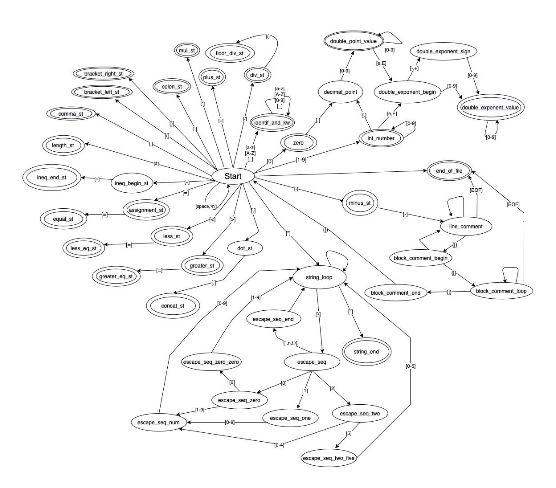
\includegraphics[width=0.95\linewidth]{finite_lexical_automat.eps}
    \caption{Deterministic finite automaton}
    \label{lexical_automat}
\end{figure}

\newpage

\section{LL grammar}
\label{LL-grammar}
\begin{enumerate}
    {\color{red}}
    \item \texttt{<intro>\arrow{}<prolog> <prog> }  
    \item \texttt{<prog>\arrow{} <fce\_decl> <prog>}
    \item \texttt{<prog>\arrow{} <fce\_def> <prog>}
    \item \texttt{<prog>\arrow{} \term{identif} <call\_fce> <prog>}
    \item \texttt{<prog>\arrow{} $\epsilon$}    
    \item \texttt{<prolog>\arrow{}\term{require} \term{''ifj21''}   }
    \item \texttt{<fce\_decl>\arrow{}\term{global} \term{identif} \term{:} \term{function} \term{$($} <type\_list> \term{$)$} <ret\_list>}
    \item \texttt{<type\_list>\arrow{}$\epsilon$}
    \item \texttt{<type\_list>\arrow{}<type><type\_list2>}
    \item \texttt{<type\_list2>\arrow{}\term{,}<type><type\_list2>} 
    \item \texttt{<type\_list2>\arrow{}$\epsilon$}
    \item \texttt{<ret\_list>\arrow{}\term{:} <type><type\_list2>}
    \item \texttt{<ret\_list>\arrow{}$\epsilon$}
    \item \texttt{<fce\_def>\arrow{}\term{function} \term{identif} \term{$($} <param\_def\_list> \term{$)$} <ret\_list> <st\_list> \term{end}}
    \item \texttt{<param\_def\_list>\arrow{}$\epsilon$}
    \item \texttt{<param\_def\_list>\arrow{}<param> <param\_def\_list2>}
    \item \texttt{<param\_def\_list2>\arrow{}\term{,}<param> <param\_def\_list2>}
    \item \texttt{<param\_def\_list2>\arrow{}$\epsilon$}
    \item \texttt{<param>\arrow{}\term{identif} \term{:} <type>}
    \item \texttt{<st\_list>\arrow{}<statement> <st\_list>}
    \item \texttt{<st\_list>\arrow{}$\epsilon$}
    \item \texttt{<statement>\arrow{}\term{local} \term{identif}\term{:}<type><init>}
    \item \texttt{<init>\arrow{}$\epsilon$}
    \item \texttt{<init>\arrow{}\term{=}<init2>}
    \item \texttt{<init2>\arrow{}\term{identif}<call\_fce>}
    \item \texttt{<init2>\arrow{}<expression>}
    \item \texttt{<statement>\arrow \term{identif} <after\_id>}    %26
    \item \texttt{<after\_id>\arrow{}<call\_fce>}
    \item \texttt{<after\_id>\arrow{}<identif\_list> \term{=} <assignment>}  
    \item \texttt{<identif\_list>\arrow{}\term{,} \term{identif}<identif\_list>}
    \item \texttt{<identif\_list>\arrow{}$\epsilon$}
    \item \texttt{<assignment>\arrow{}<expression><expression\_list2>}
    \item \texttt{<assignment>\arrow{}\term{identif}<call\_fce>} 
    \item \texttt{<expression\_list>\arrow{}<expression><expression\_list2>}
    \item \texttt{<expression\_list>\arrow{}$\epsilon$}
    \item \texttt{<expression\_list2>\arrow{}\term{,}<expression><expression\_list2>}
    \item \texttt{<expression\_list2>\arrow{}$\epsilon$}
    \item \texttt{<statement>\arrow{}\term{if}<expression>\term{then}<st\_list>\term{else}<st\_list>\term{end}}
    \item \texttt{<statement>\arrow{}\term{while}<expression>\term{do}<st\_list>\term{end}}     
    \item \texttt{<st\_list>\arrow{}\term{return}<expression\_list>}
    \item \texttt{<call\_fce>\arrow{}\term{$($} <value\_list> \term{$)$}}
    \item \texttt{<value\_list>\arrow{}$\epsilon$}
    \item \texttt{<value\_list>\arrow{}<value><value\_list2>}
    \item \texttt{<value\_list2>\arrow{}\term{,}<value><value\_list2>}
    \item \texttt{<value\_list2>\arrow{}$\epsilon$}
    \item \texttt{<value>\arrow{\term{integer\_value}}}
    \item \texttt{<value>\arrow{\term{number\_value}}}
    \item \texttt{<value>\arrow{\term{string\_value}}}
    \item \texttt{<value>\arrow{\term{identif}}}
    \item \texttt{<value>\arrow{\term{nil}}}
    \item \texttt{<type>\arrow{}\term{integer}}
    \item \texttt{<type>\arrow{}\term{number}}
    \item \texttt{<type>\arrow{}\term{string}}
\end{enumerate}

\begin{landscape}
    \section{LL\ --\ table}
    \begin{figure}[ht]
        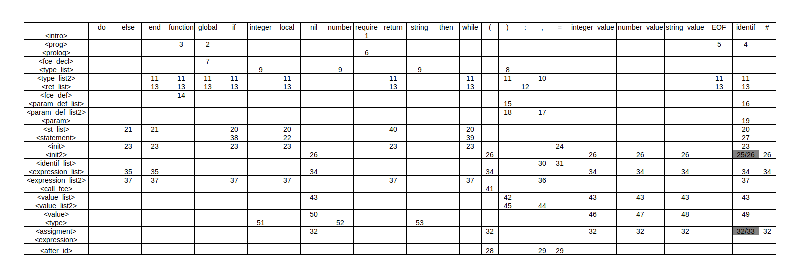
\includegraphics[scale=1.89]{LL_tabulka.eps} 
        \label{LL-table}
        \caption{LL\,--\,table  created from LL(1) grammar\\There are 2 places, where we can not decide only on LL(1) grammar, here we use semantics check for help}
    \end{figure}
\end{landscape}

\bibliographystyle{czechiso}
\bibliography{zdroje}
\end{document} 

\begin{comment}
    \section{Lex analyza}
    \subsection{FOR COPY}
    \texttt{
    <intro>     \\
    <prog>      \\
    <prolog>    \\
    <fce\_decl>     \\
    <type\_list>    \\
    <type\_list2>   \\
    <ret\_list>     \\
    <fce\_def>      \\ 
    <param\_def\_list>      \\
    <param\_def\_list2>     \\
    <param>     \\
    <st\_list>  \\
    <statement> \\
    <init>      \\
    <init2>     \\
    <after\_id>  \\
    <identif\_list>     \\ here
    <expression\_list>    \\
    <expression\_list2>     \\
    <call\_fce>         \\
    <value\_list>       \\
    <value\_list2>  \\
    <value>     \\
    <type>  \\
    <assignment> \\  
    <expression>
    }   
\end{comment}
